\documentclass{article}
\usepackage{tikz}
\usetikzlibrary{quantikz}

\begin{document}

\begin{figure}[h]
    \centering
    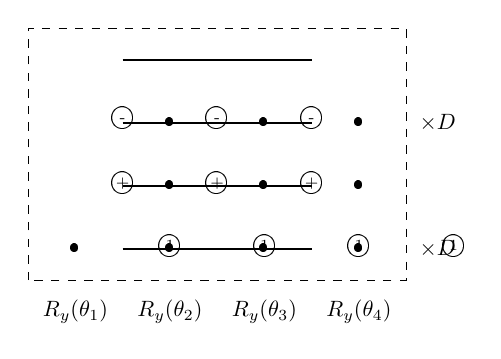
\begin{tikzpicture}[scale=0.8]
        % Draw the dashed box
        \draw[dashed] (0,0) rectangle (6,4);
        
        % Draw the qubits
        \foreach \i in {1,...,4} {
            \node[scale=0.8] at (\i*1.5-0.75,-0.5) {$R_y(\theta_{\i})$};
            \node[scale=0.8] at (\i*1.5-0.75,0.5) {\textbullet};
            \node[scale=0.8] at (\i*1.5+0.75,0.5) {\textcircled{\scriptsize 1}};
        }
        
        % Draw the Hadamard gates
        \foreach \i in {1,...,3} {
            \node[scale=0.8] at (\i*1.5,1.5) {\textcircled{\scriptsize +}};
            \node[scale=0.8] at (\i*1.5,2.5) {\textcircled{\scriptsize -}};
        }
        
        % Draw the controlled-NOT gates
        \foreach \i in {1,...,3} {
            \node[scale=0.8] at (\i*1.5+0.75,1.5) {\textbullet};
            \node[scale=0.8] at (\i*1.5+0.75,2.5) {\textbullet};
        }
        
        % Draw the control lines
        \draw[thick] (1.5,0.5) -- (4.5,0.5);
        \draw[thick] (1.5,1.5) -- (4.5,1.5);
        \draw[thick] (1.5,2.5) -- (4.5,2.5);
        \draw[thick] (1.5,3.5) -- (4.5,3.5);
        
        % Add the caption
        \node[scale=0.8] at (6.5,0.5) {$\times D$};
        \node[scale=0.8] at (6.5,2.5) {$\times D$};
    \end{tikzpicture}
    
    \caption{An example of BasicEntangler ansatz. $R_y(\theta_i)$ is a rotation gate around the y-axis by an angle $\theta_i$ applied to the i-th qubit, where $i=1,2,3,4$. The circuit layer in the dashed box can be repeated $D$ times to increase the representational capacity of the ansatz.}
\end{figure}

\end{document}